L'avvento del web 2.0 ha visto la nascita di un numero sempre crescente di servizi che permettono agli utenti di pubblicare e condividere i propri contenuti in rete. Ognuna di queste applicazioni necessita di dati identificativi dell'utente, al fine di garantire a quest'ultimo, l'accesso alle proprie risorse. 

Con il sistema di autenticazione standard, viene chiesto ad ogni utilizzatore di fornire uno \textit{username} e una \textit{password} per associare la propria identit� ad uno specifico \textit{account}. Il grande numero di servizi disponibili, per�, obbliga gli utenti a dover gestire molte informazioni di autenticazione. Accade spesso che tali utenti utilizzino la stessa password per servizi differenti, con un evidente rischio per la sicurezza.

Molte automobili di lusso possiedono una chiave per il posteggiatore. Una chiave speciale, che permette di attivare un numero limitato di funzionalit� dell'autovettura e di guidarla entro uno spazio limitato.

OAuth � un protocollo standard per autorizzazioni che, in modo simile a quanto succede per le chiavi posteggiatore per le automobili, permette ad un utente di garantire, ad applicazioni di terze parti, l'accesso ad un numero limitato di  contenuti personali.

Con OAuth inoltre gli utenti non devono condividere la propria password con diversi sistemi, bens� un server centrale di autorizzazione, funge da garante per l'identificazione delle informazioni di accesso e per la fruizione di specifici dati utente. Dal punto di vista tecnico, il protocollo � implementato utilizzando un sistema di reindirizzamenti HTTP e di controlli da parte del server che funge da garante.

Mole.io si configura al pari di altri servizi presenti sul web e, in maniera simile, sfrutta il protocollo OAuth 2.0 per l'identificazione e l'autenticazione degli utenti. In questo caso il server scelto come garante delle identit� utente � quello messo a disposizione da Twitter.

Nello schema \ref{fig:oauth2} � possibile vedere le diverse fasi del processo di autenticazione di un utente che richiede l'accesso a Mole.io.
\begin{enumerate}
\item l'utente richiede l'accesso a Mole.io;
\item l'applicazione esegue un \textit{redirect} HTTP verso la pagina di autenticazione fornita da Twitter, passandole un \textit{token} per l'identificazione dell'utente;
\item il server di autenticazione di Twitter esegue la verifica di identit� dell'utente e, in caso di esisto positivo, esegue un reindirizzamento verso un URL fornito dall'applicazione restituendo il token identificativo e un codice di verifica dell'utente;
\item a questo punto l'applicazione ottiene i dati dell'utente e pu� ritenere l'operazione di accesso effettuata con successo.
\end{enumerate}

\begin{figure}[h]
\centering
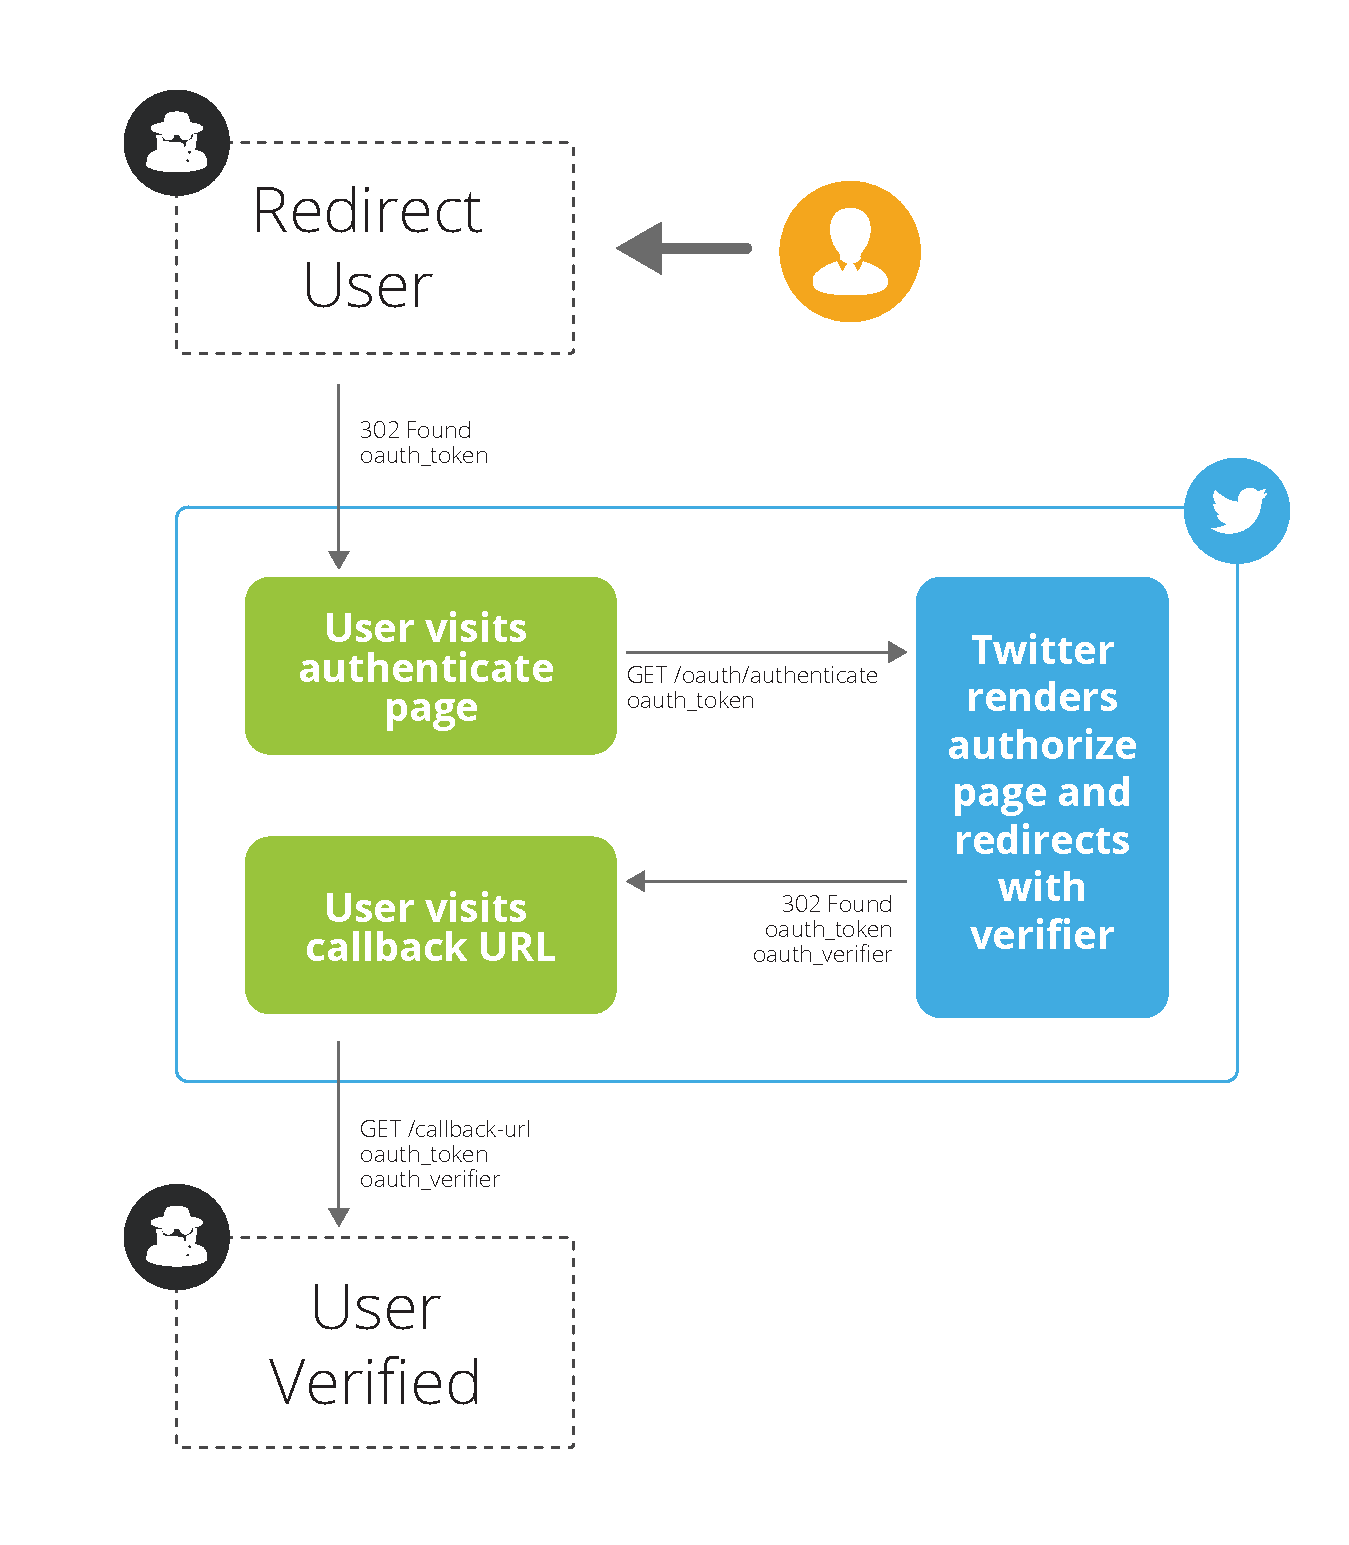
\includegraphics[width=1.0\linewidth]{./img/oauth2}
\caption[Schema di autenticazione con protocollo OAuth 2.0]{Schema di autenticazione con protocollo OAuth 2.0}
\label{fig:oauth2}
\end{figure}

%OAuth � un protocollo standard per autorizzazioni. Esso permette ad un sistema client di accedere ad una risorsa presente all'interno di un server per conto di un utente che possiede tale risorsa. Permette quindi agli utenti di garantire l'accesso, da parte di applicazioni di terzi, a dati privati presenti su un server di loro fiducia. Il vantaggio di questo tipo di protocollo � che l'utente non deve mai inserire le proprie credenziali nel sistema di terze parti, ma esclusivamente confermare la richiesta di condivisione dei propri dati al nuovo richiedente. L'autenticazione avviene utilizzando un sistema di redirezioni HTTP.

L'implementazione dell'autenticazione OAuth 2.0 all'interno di mole-suit � stata realizzata utilizzando il modulo Passport per Node.js, introdotto nella sezione \ref{Npm_e_moduli}. Passport sfrutta il sistema di middleware offerto da Express per garantire un controllo di accesso a livello di singola rotta, fornendo quindi una granularit� molto fine.

Il listato seguente � la porzione di codice, estratta da mole-suit, che implementa la procedura di autenticazione utilizzando Passport.
\begin{verbatim}
var passport = require('passport'), 
    TwitterStrategy = require('passport-twitter').Strategy;

passport.use(new TwitterStrategy({
    consumerKey: TWITTER_CONSUMER_KEY,
    consumerSecret: TWITTER_CONSUMER_SECRET,
    callbackURL: "/auth/twitter/callback"
  },
  function(token, tokenSecret, profile, done) {
    User.findOrCreate(..., function(err, user) {
      if (err) { return done(err); }
      done(null, user);
    });
  }
));

[...]

app.get('/auth/twitter', 
  passport.authenticate('twitter')
);

app.get('/auth/twitter/callback', 
  passport.authenticate('twitter', { 
    successRedirect: '/',
    failureRedirect: '/login'
  }
));
\end{verbatim}

Dopo aver importato i moduli richiesti, si configura la \textit{TwitterStrategy} di Passport, cio� la modalit� di autenticazione che permette di interagire con i server di Twitter. La configurazione prevede l'inserimento di due dati: \verb|TWITTER_CONSUMER_KEY| e \verb|TWITTER_CONSUMER_SECRET|. Questi valori sono forniti da Twitter e identificano univocamente Mole.io. Sono necessari in quanto il processo di validazione prevede che Twitter sia a conoscenza, contemporaneamente, delle informazioni dell'utente e di quelle dell'applicazione di terze parti. Per completare la configurazione � richiesta infine una funzione che permette di fornire a mole-suit le informazioni relative all'utente appena autenticato.

Le successive istruzioni riguardano la configurazione delle rotte che faranno uso dell'autenticazione con Twitter. La prima dichiara che, a fronte della richiesta dell'endpoint \verb|/auth/twitter|, � necessario eseguire la procedura di autenticazione. La seconda � necessaria per validare una autenticazione: in caso di successo, l'utente viene reindirizzato verso la pagina principale di mole-suit, in caso di insuccesso, viene riproposta la pagina di \textit{login}.

A fronte di un processo di autenticazione, Passport fornisce un oggetto contenente alcune informazioni relative all'utente. Alcuni dei campi forniti sono:
\begin{itemize}
\item \textbf{provider}, il garante della procedura di autenticazione, Twitter;
\item \textbf{id}, l'identificativo utente all'interno dei server di Twitter;
\item \textbf{displayName}, il nome dell'utente da mostrare a video;
\item \textbf{photos}, un elenco di \textit{avatar} dell'utente;
\end{itemize}  

% passport strategy (� una "base" modificata)
% va usato https

% autenticazione sull'api(?) 
% come funziona la storia id/key per autenticarsi sulle api
%api
